\documentclass[a4paper,10pt]{article}
%\usepackage[latin1]{inputenc} % Paquetes de idioma
\usepackage[utf8]{inputenc} % Paquetes de idioma (Este encoding toma acentos :) )
\usepackage[spanish]{babel} % Paquetes de idioma
\usepackage{graphicx} % Paquete para ingresar gráficos
\usepackage{grffile}
\usepackage{hyperref}
\usepackage{fancybox}
\usepackage{amsmath}
\usepackage{amsfonts}
\usepackage{listings}
\usepackage{float}
% Paquetes de macros de Circuitos
%\usepackage{pstricks}
\usepackage{tikz}

% Encabezado y Pié de página
\usepackage{fancyhdr} % Paquete para encabezados y pie de página
\pagestyle{fancy} % Sin esta línea no se imprimiría el encabezado en todas las páginas

\fancyhf{} %  Borra el encabezado anterior (Por defecto escribe el títutlo de la sección en la que se encuentra la hoja
\setlength{\headheight}{22.55pt}
\fancyhead[L]{
	{\textsf{Facultad de Ingenier\'ia $-$ Universidad de Buenos Aires \\ 66.44 Instrumentos Electrónicos}}
}
%\addtocounter{page}{5}
\fancyhead[R]{\thepage}

\renewcommand{\footrulewidth}{0.4pt} % Ajusta el tamaño de las líneas separadoras en el pié de página
\renewcommand{\headrulewidth}{0.4pt} % Ajusta el tamaño de las líneas separadoras en el encabezado

\fancyfoot[L]{
	{\textsf{Trabajo Pr\'actico N$^{\circ}4$}: Mediciones de impedancias} \\
	{\textsf{Integrantes: Eduardo Sanchez, Francisco Soler}}
	}
		

% Carátula del Trabajo
\title{ \author{} % Lo pongo para que el warning no moleste :p
\setlength{\unitlength}{1cm} %  Especifica la unidad de trabajo
\thispagestyle{empty}

\begin{picture}(18,0)
\put(0,0){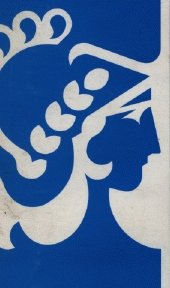
\includegraphics[width=1.5cm, height=3cm]{Logo1.png}}

\put(10.5,0){
\includegraphics[width=3cm, height=3cm]{Logo2.png}}

\end{picture}
\\[1.5cm]
\begin{center}
	\textbf{{\Huge Facultad de Ingenier\'ia \\ Universidad de Buenos Aires}}\\[2cm]
	{66.44 Instrumentos Electrónicos}\\[0.5cm]
	{Trabajo Pr\'actico N$^{\circ}3$: Mediciones de impedancias}\\[2.5cm]
\end{center}

\begin{flushleft}
	\textbf{Integrantes:} \\[1cm]

	\begin{tabular}{|c|c|c|}
		\hline
		\textbf{\normalsize Padr\'on} & \textbf{\normalsize Nombre} & \textbf{\normalsize Email} \\
		\hline
		\normalsize 92903 & \normalsize Sanchez, Eduardo Hugo & \normalsize hugo\_044@hotmail.com \\
		\hline
		\normalsize 91227 & \normalsize Soler, Jos\'e Francisco & \normalsize francisco.\_tw@hotmail.com \\
		\hline
		\normalsize xxx & \normalsize Wawrynczak, Claudio  & \normalsize claudiozak@gmail.com \\
		\hline
	\end{tabular}
\end{flushleft}
\date{} % Hace que no se imprima la fecha en la cual se compilo el .tex
 }

\begin{document}
	\maketitle % Hace que el título anterior sea el principal del documento
	\newpage

	\tableofcontents % Esta línea genera un indice a partir de las secciones y 
					 % subsecciones creadas en el documento
	\newpage


	\section{Objetivo}
	
	\indent	El objetivo del presente trabajo práctico es determinar las 
	diferentes impedancias medidas utilizando un osciloscopio con técnicas de 
	reflectometría.
	
	\newpage
	\section{Desarrollo}

	\subsection{Medición 1 - Resistencias}
	%TODO
	\indent 
	
	\subsection{Medición 2 - Bobina}
	%TODO
	
	\subsection{Medición 3 - Cortocircuito}
	%TODO

	\subsection{Medición 4 - Capacitor}
	\indent En esta medición se utilizaron 3 capacitores distintos para medir
	la resistencia y capacidad equivalente. Los valores utilizados fueron 
	$100pF$, $180pF$ y $47nF$. \\
	\indent La imagen \ref{img010} muestra las respuestas de dichas 
	mediciones. La figura de la izquierda es la respuesta del capacitor de 
	$100pF$, la del medio posee uno de $180pF$ y la de la derecha $47nF$. \\
	
		\begin{figure}[!htb]
			\centering
			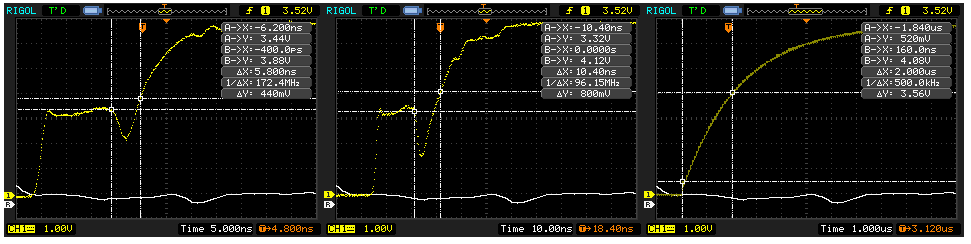
\includegraphics[width=12cm]
			{Imagenes/CurvasCapacitor.png}
			\caption{Respuestas de los distintos capacitores}
			\label{img010} 
		\end{figure}

	\indent Para poder determinar el capacitor y ressitencia equivalente lo 
	primero que se hace es determinar el tiempo de crecimiento $\tau$. El cual
	posee la siguiente fórmula

		\begin{equation}
			\tau = R\cdot C
		\end{equation}
	
	\indent La línea de transmisión posee una impedancia característica de 
	$50\omega$. Se desprecia la resistencia interna del capacitor. \\
	\indent Despejando el valor de C, en la tabla \ref{tab002} se reflejan los 
	resultados calculados con su respectivas incertidumbres. \\

		\begin{table}[!htp]
			\centering
			\begin{tabular}{|c|c|c|c|c|}
				\hline
    			C teórico & $\tau$ medido & error relativo osciloscopio & C medido &
				$\Delta$C \\
				\hline
				100 pF & $5.8~\text{n seg}$ &  & 120 pF & \\
				\hline 
				180 pF & $10.4~\text{n seg}$ & & 200 pF & \\
				\hline
				47 nF & $2~\mu\text{seg}$ & & 40 nF & \\
				\hline
			\end{tabular}
			\caption{Capacitancias medidas} 
			\label{tab002} %TODO corregir el valor de la tabla y terminar de armarla
		\end{table}

	\newpage
	\section{Colcusiones}
	%TODO
\end{document}

